\documentclass{article}
\usepackage{graphicx}
\graphicspath{{images/}}
\usepackage[utf8]{inputenc}
\usepackage{chngcntr}
\usepackage{cancel}
\counterwithin{equation}{section}

\title{Problem set 1 (Astrophysics)}
\author{Michael Nameika}

\begin{document}

\maketitle

\section{}

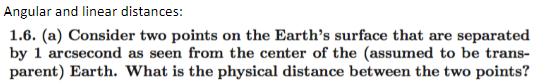
\includegraphics[scale = 0.8]{problemset1q1.PNG}
\newline\newline

To begin, first note that 

\begin{equation}
    1\:arcsecond = \frac{1}{3600}^{\circ}
\end{equation} 

And recall that there are $2\pi$ radians per $360^{\circ}$ 
\newline

Then, to convert from arcseconds to radians, simply multiply (1.1) by $\frac{2\pi}{360^{\circ}}$
\newline

Which results in

\begin{center}
    $1\:arcsecond = (\frac{1}{3600}^{\circ})(\frac{2\pi}{360^{\circ}})$
\end{center}

\begin{equation}
    \approx4.848\times10^{-6}\:rad\footnote{For the entirety of this assignment, I will be using four-digit rounding arithmetic.}
\end{equation}

Now recall the formula for arc length:

\begin{equation}
    s = r\theta
\end{equation}

Where s is the arc length, r is the radius, and theta is the subtended angle in radians.
\newline

Using the value $r = 6.371\times10^{6}$ meters for the radius of Earth, and plugging (1.2) in for $\theta$ and $r$ into equation (1.3), we get the following for the arclength:

\begin{center}
    $s = (6.371\times10^{6}\:m)(4.848\times10^{-6}\:rad)$
    \newline
    $\approx 30.89\: m$
\end{center}

Thus, the physical distance between two points on Earth's surface separated by 1 arcsecond have a physical distance of approximately $30.89\:m$.
\newline\newline

\section{}
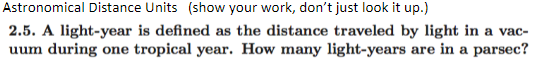
\includegraphics[scale = 0.8]{problemset1q2.PNG}
\newline\newline

Let's begin by finding how many seconds are in a sidereal year:
\begin{center}
    $t = (365.25\:\cancel{days})(24\:\frac{\cancel{h}}{\cancel{day}})(60\:\frac{\cancel{min}}{\cancel{h}})(60\:\frac{s}{\cancel{min}})$
\end{center}
\begin{equation}
    \approx3.156\times10^{7}\:s
\end{equation}
\newline
And recall the speed of light (in a vacuum):
\begin{equation}
    c = 3.000\times10^{8}\:\frac{m}{s}
\end{equation}

Now, let's find how many meters are in a light year by multiplying (2.1) by (2.2):

\begin{center}
    $1\:ly = (3.0000\times10^{8}\:\frac{m}{\cancel{s}})(3.156\times10^{7}\:\cancel{s})$
\end{center}

\begin{equation}
    \approx 9.468\times10^{15}\:m
\end{equation}

Now we have the amount of meters in a light year. Let's calculate how many meters are in a parsec and take the ratio between the amount of meters in a light year and parsec to find how many light years are in a parsec.
\newline\newline
In the following diagram\footnote{I made this diagram in MS Paint.}, when $\theta = 1\: arcsecond$, $d = 1\: parsec$ given $R$ is the average distance between the Earth and the Sun.
\newline
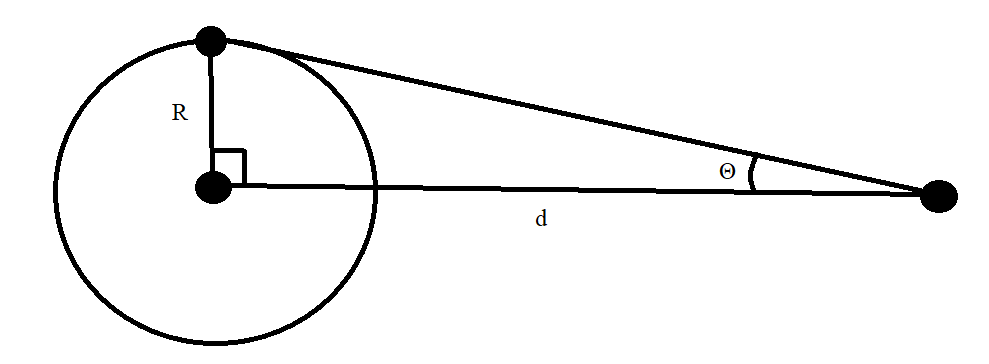
\includegraphics[scale = 0.5]{parsec diagram.png}
\newline

Given the average distance between the Earth and the Sun is 
\begin{equation}
    R = 1.500\times10^{11}\:m
\end{equation}
From the above diagram, it is clear we can use the law of sines and equation (2.4) to find that 

\begin{center}
    $1\:pc = 1.500\times10^{11}\:m(\frac{sin(90^{\circ}-\frac{1}{3600}^{\circ})}{sin(\frac{1}{3600}^{\circ})})$
\end{center}

\begin{equation}
    \approx 3.094\times10^{16}\:m
\end{equation}

Finally, we can find how many light years are in one parsec by simply finding the ratio between a parsec and a light year. That is, the ratio between equations (2.5) and (2.3):
\begin{equation}
    \frac{1\:pc}{1\:ly} = \frac{3.094\times10^{16}\:\cancel{m}}{9.468\times10^{15}\:\cancel{m}}
    \approx 3.268
\end{equation}
So there are approximately 3.268 light years in a parsec.
\section{}
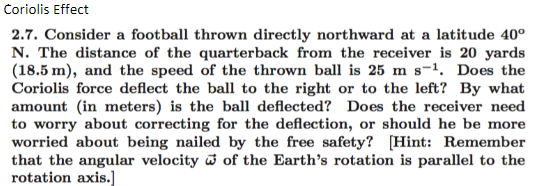
\includegraphics[scale = 0.8]{problemset1q3.PNG}
\newline\newline
The football is thrown at $40^{\circ}\: N$ with a velocity of $25\:\frac{m}{s}$
Consider the diagram below. 
\newline
\begin{center}
    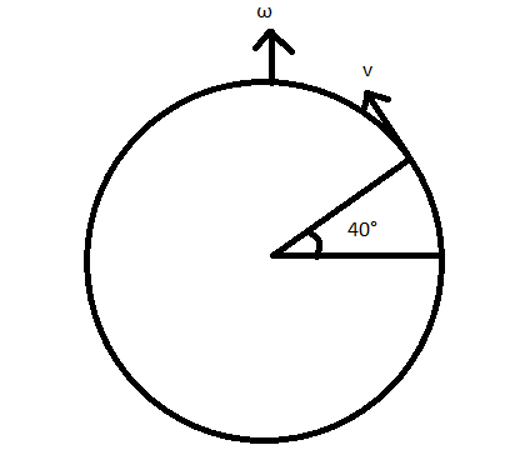
\includegraphics[scale = 0.6]{problem5diagram.png}
\end{center}
Using the sidereal day of $23\:h 56\:m$ find that
\begin{equation}
    \vec{\omega} = \frac{2\pi}{86160}s^{-1}\hat{y}
\end{equation}

And since the ball is being thrown to a target $18.5\:m$ away, we can calculate the amount of time the ball is in the air:
\begin{equation}
    t = \frac{18.5\:\cancel{m}}{25\:\cancel{m}*s^{-1}} = 0.7400\:s
\end{equation}
Now, from the equation of Coriolis acceleration,
\begin{equation}
    a_{cor} = -2(\vec{\omega}\times\vec{v})
\end{equation}
We can say that the drift of the football will be to the left of where the quarterback was aiming, from his perspective. Now we just need to find the magnitude of the Coriolis acceleration vector (since we know the direction).
\newline
Well, we know that the velocity vector will make an angle of $40^{\circ}$ with $\vec{\omega}$.
\newline\newline
To find the magnitude of the Coriolis acceleration, recall that the magnitude of the acceleration is given by 
\begin{equation}
    |a_{cor}| = 2|\omega||v|sin(40^{\circ})
\end{equation}
Clearly,
\begin{equation}
    |v| = 25\:\frac{m}{s}
\end{equation}
And plugging (3.1), and (3.5) into (3.4), we will get the following:

\begin{equation}
    |a_{cor}| = \frac{2\pi*25\:\frac{m}{s}}{86160\:s}sin(40^{\circ})\approx 1.172\times10^{-3}\:\frac{m}{s^2}
\end{equation}
Now, to find the approximate drift distance, let us use the approximate distance formula as follows:
\begin{equation}
    d \approx \frac{1}{2}a_{cor}t^2
\end{equation}
Plugging in (3.2) and (3.6) into (3.7), we will get the following:
\begin{center}
    $d \approx \frac{1}{2}*1.172\times10^{-3}\:\frac{m}{\cancel{s}}*(0.7400\:\cancel{s})^2$
\end{center}
\begin{equation}
    \approx 3.209\times10^{-4}\:m
\end{equation}


So the drift due to the Coriolis effect on the football will be approximately $3.209\times10^{-4} \: m$
\newline
I would say it's a safe assumption that the receiver does not need to worry about correcting for the deflection.

\section{}
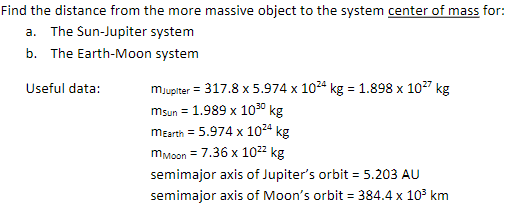
\includegraphics[scale = 0.8]{problemset1q4.PNG}
\newline\newline
To find the center of mass between the Sun and Jupiter, let's use the following equation:
\begin{equation}
    r_{com} = \frac{m_1}{m_1+m_2}r
\end{equation}
Which gives us the distance from $m_2$ to $m_1$. In our case, let $m_2$ be the mass of the Sun and $m_1$ be the mass of Jupiter. From the table above,
\begin{equation}
    m_{Jupiter} = 1.898\times10^{27}\:kg
\end{equation}
\begin{equation}
    m_{Sun} = 1.989\times10^{30}\:kg\
\end{equation}
With the distance between the Sun and Jupiter as given:
\begin{equation}
    r_{Sun/Jupiter} = 7.784\times10^{11}m
\end{equation}
Plugging (4.2), (4.3), and (4.4) into (4.1), we get the following:
\begin{center}
    $r_{com} = (\frac{1.898\times10^{27}\:\cancel{kg}}{1.898\times10^{27}\:\cancel{kg} + 1.989\times10^{30}\:\cancel{kg}})7.784\times10^{11}\:m $
\end{center}
\begin{equation}
    \approx 7.421\times10^{8}\:m
\end{equation}
Thus, from (4.5), the common center of mass between the Sun and Jupiter is approximately $7.421\times10^8\:m$ from the center of the Sun.
\newline\newline
Now, for the center of mass of the Earth-Moon system: From the table above, the mass of the Earth and the Moon are, respectively,
\begin{equation}
    m_{Earth} = 5.974\times10^{24}\:kg
\end{equation}
\begin{equation}
    m_{Moon} = 7.360\times10^{22}\:kg
\end{equation}
Where the semi-major axis of the Moon's orbit around the Earth is given by:
\begin{equation}
    r_{Earth/Moon} = 3.844\times10^{8}\:m
\end{equation}
Now, plugging (4.6), (4.7), and (4.8) into (4.1), we get the following:
\begin{center}
    $r_{com} = (\frac{7.360\times10^{22}\:\cancel{kg}}{7.360\times10^{22}\:\cancel{kg} + 5.974\times10^{24}\:\cancel{kg}})3.844\times10^8\:m$
\end{center}
\begin{equation}
    \approx 4.678\times10^6\:m
\end{equation}
Thus, by (4.9), the center of mass of the Earth-Moon system is approximately $4.678\times10^6$ meters from the center of the Earth.



\section{}
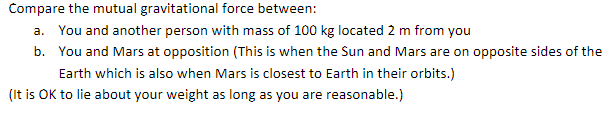
\includegraphics[scale = 0.8]{problemset1q5.PNG}
Recall Newton's law of gravitation:
\begin{equation}
    F_{grav} = G\frac{m_1m_2}{r^2}
\end{equation}
Where G is given by:
\begin{equation}
    G = 6.670\times10^{-11}\:\frac{Nm^2}{kg^2}
\end{equation}
Now let $m_2 = 100\:kg$ and $m_1 = 80.74\: kg$ (my mass)
\newline
Now plugging in (5.2), $m_1$, $m_2$, and $r = 2\:m$ into (5.1), we will get:
\begin{center}
    $F_{m_1m_2} = 6.670\times10^{-11}\:\frac{N\cancel{m^2}}{\cancel{kg^2}}(\frac{80.74\:\cancel{kg}*100.0\:\cancel{kg}}{(2.000\:\cancel{m})^2})$
\end{center}
\begin{equation}
    \approx 1.346\times10^{-7}\:N
\end{equation}



Thus the force of gravity between me and a person of mass $100\: kg$ standing $2\:m$ away from me is approximately $1.346\times10^{-7}\:N$, as given by (5.3).
\newline\newline
Now, let's find the force of gravity between me and Mars at opposition.
First note that the mass of Mars is:
\begin{equation}
    m_{Mars} = 6.390\times10^{23}\:kg
\end{equation}
And that the distance between Earth and Mars at opposition is:
\begin{equation}
    d_{Earth Mars} = 6.207\times10^{10}\:m
\end{equation}

Now, let's plug in (5.4), (5.5), (5.2), and my mass into (5.1) to find the mutual force of gravity between me and Mars at opposition:
\begin{center}
    $F_{Me, Mars} = 6.67\times10^{-11}\:\frac{N\cancel{m^2}}{\cancel{kg^2}}(\frac{80.74\:\cancel{kg}*6.39\times10^{23}\:\cancel{kg}}{(6.207\times10^{10}\:\cancel{m})^2})$
\end{center}
\begin{equation}
     \approx 8.932\times10^{-7}\:N
\end{equation}
Thus, the mutual gravitational force between me and Mars at opposition is approximately $8.932\times10^{-7}\:N$, as given by (5.6).

\section{}
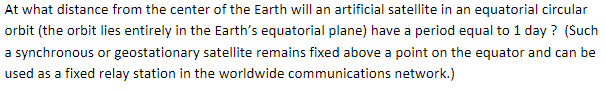
\includegraphics[scale = 0.8]{problemset1q6.PNG}
\newline\newline
Recall Kepler's third law:
\begin{equation}
    P^2 = \frac{4\pi^2}{G(m_1+m_2)}a^3
\end{equation}
Where $P$ is the period, $a$ is the semi-major axis, and $G$ is given in equation (5.2).
\newline
Now let $m_1$ be Earth's mass and $m_2$ be the mass of the satellite. It goes without saying that the mass of the Earth is going to be much, much larger than the mass of the satellite, so we can approximate Kepler's third law as
\begin{equation}
    P^2 \approx \frac{4\pi^2}{Gm_1}a^3
\end{equation}
We wish to solve for $a$, so rearranging (6.2) into terms of $a$ gives us
\begin{equation}
    a \approx (\frac{P^2*G*m_1}{4\pi^2})^{\frac{1}{3}}
\end{equation}


For the satellite to be geosynchronous, we want the period of its orbit to be equal to the period of Earth's rotation, For this calculation, I will use a sidereal day, for which the period is 
\begin{equation}
    P = 86160\:s
\end{equation}


Given that the mass of the Earth is
\\[20pt]
\begin{center}
    $m_1 = 5.972\times10^{24}\:kg$
\end{center}
and plugging this along with (5.2), (6.4) into (6.3), we get the following:
\begin{center}
    $a \approx (\frac{(86160\:\cancel{s})^2*6.67\times10^{-11}\:\frac{m^3}{\cancel{kg}*\cancel{s^2}}*5.972\times10^{24}\:\cancel{kg}}{4\pi^2})^{\frac{1}{3}}$
\end{center}
\begin{equation}
    \approx 4.215\times10^7\:m
\end{equation}
Thus, the radius of a geosynchronous orbit of a satellite for Earth is approximately $4.215\times10^7\: m$ from the center of the Earth, as given by (6.5).

\end{document}